\section{Szoftver vezérlő rész}

\subsection{A beépített ADC használata}

A mikorvezérlőbe egy 3 csatornás ADC van beépítve, viszont egyszerre csak 1 
csatornát lehet olvasni, olvasás előtt át kell váltani arra a csatornára, amelyről
az adatot olvasni akarjuk. Az ADC hardver szinten egy 48Mhz-es órajelet kap és
egy mérés minimum 96 ciklusba telik, így 500k mérést végez másodpercenként, 
ezt viszont növelhető dinamikusan szoftveresen, így csökkenthető a mérési gyorsaság.


Az ADC képes DMA-n (direct memory access) \cite{DMA} keresztül kommunikálni a 
memóriával, így inicializálás után automatikusan elvégzi a méréseket az adott
csatornán. A csatorna inicializálása a következőképpen alakul. A méréseket
egy előre lefoglalt tömbbe teszi ami jelen esetben a \textbf{capture$\_$buf} tömb,
aminek a mérete \textbf{CAPTURE$\_$DEPTH} . A mérés után a tömbben időrendi sorrendben
kiolvashatók a mérések.


\begin{lstlisting}

    //ezeket csak egyszer a konstruktorban kell meghivni
    dma_chan = dma_claim_unused_channel(true);
    cfg = dma_channel_get_default_config(dma_chan);

    //minden indulas elott
    adc_fifo_setup(
        true, // Write each completed conversion to the sample FIFO
        true, // Enable DMA data request (DREQ)
        1,    // DREQ (and IRQ) asserted when at least 1 sample present
        true, // Set sample error bit on error
        false // Keep full 12 bits of each sample
    );
    //Set the size of each DMA bus transfer
    channel_config_set_transfer_data_size(&cfg, DMA_SIZE_16);
    channel_config_set_read_increment(&cfg, false);
    channel_config_set_write_increment(&cfg, true);
    channel_config_set_dreq(&cfg, DREQ_ADC);
    dma_channel_configure(dma_chan, &cfg,
                          capture_buf,   // dst
                          &adc_hw->fifo, // src
                          CAPTURE_DEPTH, // transfer count
                          true           // start immediately
    );

    // miutan elo van keszitve
    adc_run(true);//elinditja a merest
    dma_channel_wait_for_finish_blocking(dma_chan);//var mig befelyezi a merest
    adc_run(false);//leallitja a merest

\end{lstlisting}

Az ADC konstans hibával rendelkezik, vagyis 0V feszültséget nem 0-nak érzékel
és 3.3V-ot nem 4096-nek (az ADC 12 bites felbontású). Ezért erre a célra egy
lineáris hibajavító függvény van alkalmazva. Ennek működési lényege, hogy
megméri 0V-on milyen értéket mér az ADC és 3.3V-on. Ezeket az értékeket elmenti
és minden jövőbeli mérést a következőképpen korrigál.


\begin{lstlisting}
    for (int i = 0; i < samplesSize; i++)
    {
        samples[i] = (samples[i] * VCCOffset) - gndOffset;
    }
\end{lstlisting}

\subsection{Digitál analóg Konverter}

A DAC SPI-n keresztül kömmunikál, ezért
szüksége van egy SPI osztályra amely inicializálja az 
SPI portokat. A használt portok szintén a \textbf{Global.h}
fájlban találhatóak meg. A DAC szintén használ az SPI protokokolon
kívüli jeleket, viszont ezek a reseten kívül opcionálisak és 
elégséges lenne közvetlen a földre kötni. Ezekkel a jelekkel
lehetséges lenne jelet küldeni, hogy mikor töltse be az adatot
a pufferből, viszont ez szoftveresen is megoldható így azt a megoldás
van alkalmazva.

Mivel egy külső feszültség referencia van alkalmazva, így a belsőt
ki kell kapcsolni a \textbf{0x012000} parancs küldésével az SPI-n keresztül.
A küldés során 24 bitet vár a DAC amiből az első 8 bit parancsként
van értelmezve, míg a hátsó 16bit adatként. Mindenik lehetséges parancs
fel van sorolva a \textbf{IDAC.h}-ban, amit, így a parancs nevét és a 
kívánt feszültséggel kell a függvényt meghívni.

\subsection{PID szabályozó konstans áram előállítására}

A karakterisztika diagramm elkészítéséhez a tranzisztor bázisán egy konstans áram
folyik át, míg a kollectoron 0 tól 3.3V-ig növekedik a feszültség. Viszont
ez a rendszer csak NPN típusú tranzisztoroknak képes kirajzolni, mivel a
PNP tranzisztoroknak negatív feszültség szükséges, hogy konstans áram legyen
a bázison, ami nem lehetséges ezzel az áramkörrel.

Mivel a rendszer nem tartalmaz egy konstans áram forrást, csak feszültséget,
így szoftveres segítségget az DAC van erre a célra felhasználva. A 
szabályozásra egy PID szabályozó van használva, melynek csak a proportional
része van használva, mivel a kimenet nem függ az múltbeli értékektől,
így a szabályozás egyszerűbb ezáltal. A választott konstans áram 
amikor a bázison és collectoron a feszültség 3.3V, ilyenkor az
áramerősség a bázison a legalacsonyabb a tesztelhető tartományban.
Ezután a bázis feszültséget szabályozva megközelíti ezt az áramerősséget
ahogy a kollector feszültség növekedik.

A a diagramm 200 mérési pontot tartalmaz és még ebben az esetben is a 
diagramm kirajzolása közel 2-3 másodpercet vesz igénybe. Ez idő alatt 
az azonosítás eredményei láthatóak a kijelzőn, így a felhasználó láthatja
a rész eredményeket miközben a mérés még folyamatban van. 
A rész eredmények tartalmazzák az eszköz láb kiosztását, a komponenst
nevét és az erősítését. A szabályozás algoritmusa a következőképpen
alakul

\begin{lstlisting}
    //a jelenlegi bazis aram
    currentBasemA = getShuntcurrent(icalculate, convertToVolt(baseVoltage), basePin);
    //hiba a jelenlegi es az elvart kozt
    error = ConstCurrentVal - currentBasemA;
    //hiba korrigalasa
    pidCorr = pid->pid_process(error);
    //pid kimenetenek skalazasa [-1,1] koze
    pidCorr = (pidCorr / maxPID);
    //korrigalt feszultseg
    reqVolt = convertToVolt(baseVoltage) + 3.3 * pidCorr;
    //amennyiben a hiba eleg alacsony a szabalyozas kilep
    if (std::abs(error) < 0.01)
        return;
    //feszultseg abszolut limiteinek meghatarozasa    
    if (reqVolt > 3.3)
        reqVolt = 3.3;
    if (reqVolt < 0)
        reqVolt = 0;
    //feszultseg kiirasa a DAC-ra
    baseVoltage = (int)((reqVolt / 3.3) * UINT16_MAX);
    setVoltageOnChannel(baseVoltage, baseCommand);
\end{lstlisting}

\subsection{Beépített SPI használata}

A mikrovezérlőnek 2 különálló SPI chatornája van és mindkét csaornának 2 különböző
helyre van kivezetése a GPIO-ra [\ref{fig:Pico_pinout}]. Itt rá kell csatlakoztatni az eszköz vezetékeit, úgy
hogy egy eszköz minden SPI vezetéke ugyan azt a csatornát használja.

Amennyiben csatlakoztatva van akkor programon belül meg kell határozni, hogy 
melyik GPIO van használva melyik célra, itt nem kötelező mind a 4 (MOSI,MISO,CLK,CS)
jeleket felsorolni, vagy akár csatlakoztatni fizikailag a MISO esetében. Az 
ajánlott a MOSI és a CLK jelek, hogy majd lehessen változtatni az SPI módokat.

Beépítetten 8 és 16 bites adat tömböt vár szoftver oldalon, viszont csak az első
8 bitet küldi el, ha a programozó nem állítsa át. Nagyobb adatot is át lehet 
küldeni (pl. 24bit amit a DAC használ), viszont azt a programozó kell megoldja,
mint egy 16 bites és egy 8 bites csomag. Ezért nem használtam a CS jelt, mint 
SPI jel, hanem digitális jel, mert így teljes kontrollom volt felette és nem 
kellett féljek, hogy ilyenkor a CS belezavar a küldésbe.


\subsection{Kijelző vezérlése}

A kijelző vezérlése a [\ref{fig:displayClassDiagram}] ábrán látható osztály diagrammot használja, 
az SPI osztálynak meg kell adni, hogy hová vannak csatlakoztatva a vezetékek, 
ezek az adatok megtalálhatóak a \textbf{Global.h} fájlban, ezen kívül a 
kijelző használ még egyedi vezérlő jeleket is, amelyek globálisan definiálva vannak,
így ezeket nem kell megadni. 

A kijelzőnek van egy DC jele, ami a parancs és adat mód váltásáért felelős.
Amennyiben ez a jel magas akkor a beérkező adat parancsként van értelmezve, amíg 
ez alacsony akkor adatként.

Nincs a teljes képernyő adata elmentve a memóriában egy időben, mivel a kijelzőnek
van saját memóriája, így csak módosítani kell azt. A memóriában egy időben csak 
egy 8 pixel magas sor van eltárolva, mivel egy karakter is ilyen magas.
Amint megvan egy sor kiszámítása akkor azt elküldi és kezdi a következő sort.
Mivel a kijelző nagy frekvenciás órajellel is képes működni (68Mhz), így a küldési
idő is alacsony.

Az ILI9341 osztály csak az inicializálásért felel, a parancs és adat 
módokban való küldésért és a képernyő teljes újratöltésére egy színnel, vagy a jelenlegi
sortól kezdve a kijelző végéig.

A CHARACTERDISPLAY osztály képes egyszerű ASCII alapú üzenetek kijelzésére.
Ezt egy mask tömbbel éri el, minden karakternek van egy 8x8as maskja, amely
bittenként tárolja el, hogy hol kell változtatni a színt.
Ahol a mask 1-es értékű, ott a pixelt a karakter színűre kell festeni, ahol 0
ott a háttérszínűre.
Ez minden betűn egyenként végig halad és beteszi a tároló tömb megfeelő indexére
a szín értéket, a tároló sor küldés kezdetekor fel van töltve a háttérszín 
értékével, ez törli az előző sor értékeit és így csak ott kell módosítani
ahol szükséges.
Küldés során printLine(string) függvény kap egy string értéket.
Itt figyelemmel kell lenni arra, hogy automatikusan nem kezd új sort
ha hosszú a szöveg. Ezen karakterenként végig haladva átalakítja a karaktereket maskokká
és beírja a tárolóba. A 


\begin{lstlisting}

void CHARACTERDISPLAY::insertChar(uint8_t position, const uint8_t *charSet)
{
    for (int bit = 0; bit < 8; bit++)
    {
        uint8_t mask = 128 >> bit; // from last in the mask to the first
        for (uint16_t i = 0; i < lineHeight; i++)
        {
            if (charSet[i] & mask)
            {
                // id is the position of the pixel
                int id = i * lineWidth + position * 8 + bit;
                row[id] = fg_Color; // set pixel to fg_Color
            }
        }
    }
}

\end{lstlisting}


A GRAPHDISPLAY képes használni a CHARACTERDISPLAY függvényeit és kibővíti azzal,
hogy lehetővé teszi XY grafikonok kirajzolását. Itt csak egy vektort kell megadni,
az szerint lesz skálázva, hogy a kijelzőt a legnagyobb mértékben kihasználja.
A kijelző legfelső sorában lesz a maximális érték és az szerint lesz skálázva a
többi érték. A kapott értékek számától függően az OX tengelyen az szerint lesznek
egyenletesen felosztva az értékek.

A függvény hívásakor meg kell adni, hogy az értékek milyen mértékegységűek, ez 2
karakter lehet maximum (pl. mA). 



\subsection{Analóg kapcsoló}

Ennek az osztálynak a feladata az analóg kapcsolók vezérlése és ez az
osztály vezérli a DAC-ot is. Ez képes egyszerre vezérelni mindhárom kapcsolót
egyszerre és mivel a komponens azonosítására nem szükséges analóg jeleket
használni, így egy beállítás táblázatot használ, amellyel megadható, hogy 
melyik ellenállást kapcsolja és, hogy milyen feszültséget adjon le a DAC
a következő táblázat szerint [\ref{fig:KapcsoloMod}].

\begin{figure}[H]
    \centering
    \begin{tabular}{|l|l|l|}
    \hline
    Mód & Használt ellenállás & Feszültség \\ \hline
    0   & Nincs               & 0V         \\ \hline
    1   & Kicsi(100 Ohm)      & 0V         \\ \hline
    2   & Kicsi(100 Ohm)      & 3.3V       \\ \hline
    3   & Közepes(330 Ohm)    & 0V         \\ \hline
    4   & Közepes(330 Ohm)    & 3.3V       \\ \hline
    5   & Nagy(4700 Ohm)      & 0V         \\ \hline
    6   & Nagy(4700 Ohm)      & 3.3V       \\ \hline
\end{tabular}
\caption{Kapcsolási táblázat}
\label{fig:KapcsoloMod}
\end{figure}

Így a mérés során csak egy 0-6 közti értéket kell küldeni 
ahhoz, hogy a megfelelő ellenállást és feszültség legyen
minden kapcsoló kimenetén. Lehetőség van arra is, hogy csak 
a feszültség legyen beállítva és a kapcsoló nyitott állapotban legyen,
ez abban az esetben fontos ahol időben való változást kell figyelni,
mint például a tranzisztor töltése. Ebben az esetben előre 
beállítható a DAC kimenete és mivel az ADC osztály a második
processzor magon fut így a szemafor jelzésére az ADC elkezd mérni, 
viszont ha ekkor kerül csak elküldésre az adat a DAC-nak akkor 
nagy késések lehetnek és az ADC hibás adatokat fog mérni.
Így ha csak a kapcsolót kell átkapcsolni akkor a késés minimális és az ADC
nem fog hibás adatokat olvasni.

Az a kapcsolók egyszerre való írása maszkolással van elérve. Mivel az 
analóg kapcsolók egymás mellett helyezkednek el, így azt a 
részt ki lehet maskolni és az érték maszkba meg azokra a pozíciókra
kerül amit be akarunk írni. Ezt a beépített gpio$\_$put$\_$masked(uint32$\_$t mask, uint32$\_$t value)
függvénnyel értem el. A Sw$\_$translation$\_$Map a [\ref{fig:KapcsoloMod}] táblázatban
szereplő értékeket tartalmazza.


\begin{lstlisting}

void ASWITCHCONTROLLER::setSwithcSetting(const uint8_t sw1, const uint8_t sw2, const uint8_t sw3)
{
    // set switch
    gpio_put_masked(this->mask, 0 | (Sw_translation_Map[sw1].setting << 16) | (Sw_translation_Map[sw2].setting << 18) | (Sw_translation_Map[sw3].setting << 20));
}

\end{lstlisting}


\section{Szoftver logikai rész}

Az azonosítás a [\ref{fig:CalculateStateDiagram}] ábrán látható
módon történik egy állapot gép osztály struktúrát alkalmazva.
A kezdetben ismeretlen komponensként van az alkatrész azonosítva,
majd ahogy egy fázison áthalad úgy frissítve lesz. 
Egy ilyen példa a tranzisztor tesztelése. Első lépésben elbukik az 
ellenállás teszten így nem lesz frissítve, majd a dióda teszten
megtalálja vagy a Collector-Bázis vagy a Bázis-Emmiter diódát, 
mivel egyszerre csak 1-et keres a tesztelés során, elmenti ezeknek az 
paramétereit, majd a tranzisztor tesztelés során fölülírja ezeket az értékeket 
és a tranzisztor értékeivel tölti fel.

Amennyiben egy következő fázis nem sikeres akkor abban az esetben 
a régi értékek megmaradnak és az lesz az azonosítás eredménye.

\subsection{Ellenállás teszt}

Az ellenállás tesztelés során ellenőrzi, hogy az eszköz teszteli, 
hogy a alkatrész az egy dióda vagy ellenállás és amellyiben ellenállás 
akkor elmenti az ellenállását. Amennyiben egyiket sem találja
akkor abban az esetben az alkatrész nem detektálható ezzel az eszközzel.

Mivel a diódáknak az a tulajdonságuk, hogy csak egyik irányban vezetnek
és áramerősségtől kevésbé függő a feszültség esésők, így fel lehet ezt
használni a detekciójukra.

Első lépésben ellenőrzi, hogy az alaktrész vezet-e mindkét irányban, 
minimális eltéréssel akkor ezzel az egyszerű dióda ki van zárva.
A tesztelés során ugyan azon irányból, csak különböző ellenállásokkal
is letesztelődik, ennek lényege az, hogy ha esetlegesen az alkatrész
egy ellenállás akkor az alkatrészen levő feszültség esés lehet olyan alacsony,
hogy az nem pontosan mérhető. 
Egy ilyen eset amikor a kapcsoló ellenállásai nagy értéküek, de a tesztelt 
ellenállás kis értékű, így
a mért feszültség esés néhány mV ami nem mérhető pontosan, így a 
mérés nem használható. 

Viszont az a lehetőség is fenn áll, hogy a tesztelt eszköz egy
inverz dióda, így ez mindkét irányban azonosan vezet, ezt a különböző
kapcsoló ellenállásokkal lehet detektálni, mivel a feszültség esés hasonló
így ezt észlelve bizonyos, hogy az alkatrész egy inverz dióa.

\begin{lstlisting}
    bool STATE::twoInverseDiode()
    {
        if (usedModes.size() < 4)
        {
            return false;
        }
        bool fw = false, bw = false;
        //check voltage drop with different resistors in forward mode
        double threshold1 = icalculate->diodeThreshold(usedModes.at(0));
        double threshold2 = icalculate->diodeThreshold(usedModes.at(2));
        if (std::abs(threshold1 - threshold2) < 0.5)
        {
            fw = true;
        }
        //check voltage drop with different resistors in reverse mode
        threshold1 = icalculate->diodeThreshold(usedModes.at(1));
        threshold2 = icalculate->diodeThreshold(usedModes.at(3));
        if (std::abs(threshold1 - threshold2) < 0.5)
        {
            bw = true;
        }
        
        return fw && bw;
    }
\end{lstlisting}


Amennyiben bizonyos, hogy az alkatrész egy ellenállás akkor
abban az esetben az kapcsoló ellenálláson eső feszültségből kiszámítható
az áram az áramkörben és mivel a feszültség esés ismert az alkatrészen,
így ebből kiszámítható annak ellenállása is.

Az áramerősséget azon az ellenálláson keresztül méri, amely 
felől az áram folyik az áramkörbe (ebben az esetben csak 1 feszültség
forrás aktív a többi földként működik).

A tesztelés során a következő áramkör alakul ki[\ref{fig:ResistorExampleCircuit}], 
itt a 2 
vízszintes ellenállás a kapcsoló ellenállás ez változtatható
és a függőleges az ismeretlen ellenállás. A 2 feszültség mérő az ADC
csatornáját szimbolizálja.

\begin{figure}[H]
    \centering
    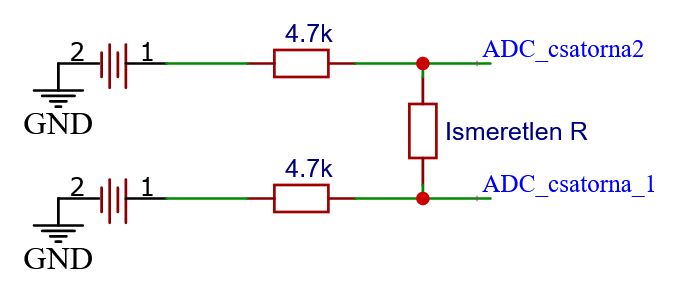
\includegraphics[scale=1]{images/diagrams/ResistorExampleCircuit.png}
    \caption{Ellenállás mérés áramköre}
    \label{fig:ResistorExampleCircuit}
\end{figure}

\subsection{Kondenzátor}

Mivel a kondenzátok ellenállás karakterisztikát mutatnak abban az esetben
amikor a 2 pólusán levő feszültséget mérjük és nem mutat 
dióda karakterisztikát ezért az ellenállás 
teszten átmegy.

A mérés a töltési időt méri egy meghatározott ellenálláson keresztül,
ebből az időből és ellenállásból határozza meg a Kondenzátor méretét.

Mivel az ADC egy állítható frekvencián mér és egy mérés során azonos ütemben
több mérést végez el (ebben az esetben 255), amelyet ebben az esetben
nem átlagol, mint a többi esetben. Így az idő meghatározható a jelenlegi
ADC frekvenciából és hogy hány mérés volt szükséges, hogy a kondenzátor
63\%-ban felteljen.

Amennyiben sikerül egy olyan módot találni (mérési frekvencia és ellenállás)
ahol a mérési puffer vége előtt feltelik 63\%-ra akkor az alapján kiszámolja
a kondenzátor méretét. Viszont 10nF alatt nem képes pontosan meghatározni,
mivel a tervezés fázis alatt nem volt elég nagy ellenállás választva
ezért a töltés túl gyors.

Minden sikertelen tesztelés után és a legelső mérés előtt kondenzátort kisüti, 
hogy a következő mérést ne befolyásolja. Ha félig fel lenne töltve a kondenzátor
akkor a következő mérés alatt sokkal hamarább elérné a küszüb feszültséget
a kellett időnél így hibás értéket számolna ki.



\subsection{Dióda teszt}

Amennyiben az ellenállás teszt során erre az útvonalra kerül
abban az esetben kiszámolja a nyitó feszültség értékét.
Mivel előző lépésben mért értékek el vannak mentve, így ebben 
az esetben fel lehet használni azokat és nem kell ugyan azt a 
mérést elvégezni.

Ez a lépés meghatározza a dióda feszültség esését az által, hogy a 
dióda 2 végén levő feszültség értékeket kivonva egymásból.
Ezt mindkét irányban megméri és amennyiben a dióda nyitó
feszültsége 3V alatt van akkor abban az esetben képes megmérni azt.

Attól függően, hogy melyik irányból folyik az áram meghatározza
a dióa anód/katód pólusait is, amennyiben az alkatrész egy 
2 inverz dióda akkor abban az esetben a mindkét pólusra 
Anód-Katód azonosítást ad.

Ez a lépés után következik a tranzisztor tesztelés, mivel a
tranzisztorok tartalmaznak diódát így erről a fázisról képes eljutni.

\subsection{Tranzisztor teszt}

Ebben a fázisban tesztelésre kerül, hogy a komponens NPN vagy PNP tranzisztor.
A tesztelés során meg lesz határozva a tranzisztor erősítése és hogy 
melyik a tranzisztor láb kiosztását a Collector-Emmiter különbséget is figyelembe
véve.

PNP tranzisztor esetében a bázist földre kell kötni, hogy a tranzisztor kinyisson.
Ebben az esetben a tranzisztor Collector-Emmiter és Emmiter-Collector irányban
is vezet. A mérés megismétlődik NPN tranzisztor módra is, ebben az esetben 
a Bázisra feszültséget kell kapcsolni, hogy kinyisson és ez is mindkét irányban
vezet.

Amennyiben mindkét teszt sikeres (NPN és PNP) akkor a teszt sikertelen, mivel
egyszerre nem lehet mindkettő. Amennyiben csak az egyik teszt sikeres akkor
abban az esetben megméri a tranzisztor erősítését Collector-Emmiter és 
Emmiter-Collector irányban. A teszter nem tudja ezeket, csak az egyszerűség
kedvéért van ilyen módon leírva. Mindkét esetben kijön egy-egy erősítés érték,
viszont amikor az áram a Collector-Emmiter úton halad akkor abban az esetben
az erősítés sokkal nagyobb, mint fordított irányban így meghatározható a 
Collector és Emmiter láb.

A tranzisztor erősítése az ellenállás mérés alatt bemutatott áramerősség
mérésen alapul. Az áramerősséget megméri a Bázison és a Collectoron keresztül
és ennek \textbf{Ic/IB} aránya adja meg az erősítést. Ic ebben az esetben mindig
az a láb amely felől az áram folyik.

A karakterisztika diagramm elkészítéséhez első lépésben a tranzisztor azonosítása
szükséges, mivel itt szükséges a tranzisztor lábkiosztásának az ismerete.
A PID vezérlő konstans áramot enged át a tranzisztor bázisán bármilyen
Kollector-Emmiter feszültség mellett. 

Az NPN tranzisztoroknál a bázis feszültség
magasabb kell legyen, mint a tranzisztor Emmiter feszültsége.
Ez lehetséges a mérés teljes tartományban, mivel az Emmiteren a feszültség
mindig alacsonyabb, mint a Bázison, így csak a Bázis feszültségét kell
szabályozni.

A PNP tranzisztor esetében a bázis feszültség alacsonyabb kell legyen,
mint az emmiter feszültség. Ezen esetben a Bázis feszültség lehetséges 
lenne, hogy negatív értékeket vegyen fel, amit a DAC nem képes szolgáltatni.
Viszont virtuális negatív feszültség elérhető, így a mérés elvégezhető 
a következő módon. Az Emmitert egy konstans 3.3V feszültségen tartva a
Kollectort növelve a Kollector-Emmiter feszültség csökken, miközben
relatív negatív feszültség érhető el a bázison.
Ennek segítségével a teljes mérési tartományon mérhető, annélkül,
hogy a bázisra a DAC-hoz képest negatív feszültségre lenne szükség.



%----------------------------------------HW-------------------------

\section{Hardver rész}

A rendszer elkészítéséhez szükséges volt egy áramkör tervezése is, mivel több komponens
csak SMD (Surface Mount Component) formában találhatóak meg, így nem alkalmazhatóak egy
egyszerű breadboard. Ezen megtalálható minden ami szükséges a rendszer működéséhez, 
csupán egy micro-USB szükséges a rendszer táplálásához.

Az áramkör tervet az EasyEDA-ban terveztem, ez egy ingyenesen használható szerkesztő
program, akár webes felületen is használható és nagy mennyiségű alkatrész található
meg az adatbázisában amelyek a tervezésre használhatóak.

Az áramkör egy kétoldalas lapon található és csak egy oldalán találhatóak a komponensek.
A másik oldalán legfőképpen a huzalozás található. A rendszer használ kis méretű
SMD alkatrészeket és THC alkatrészeket is. 

A huzalozás során nagyobb figyelmet fektettem a nagy frekvenciás SPI jelek
és a mérőáramkör szétválasztására, a zajok csökkentése érdekében.

A jel vezető huzalok vékonyabbak, mint az áramot vezető huzalok, viszont ez csak
design szempontjából van jelentősége, mivel az áramerősség alacsony így vékonyabb
hozalok is megfelenének a feladatra. Egyes esetekben amikor a kis méretű SMD 
alkatrészekhez kell csatlakoztatni a vezetékeket akkor közvetlen a csatlakoztatás
előtt a vezeték vastagság lecsökken, hogy lehetséges legyen a forrasztás annálkül,
hogy a mellette levő lábbal rövidzárt okozzon.

A chipek mellett találhatóak kondenzátorok is, amelyek a tápfeszültség stabilitására
szolgálnak.

\subsection{Problémák az áramkör tervezésekor}

Mivel számomra az áramkör tervezés tárgy nem volt elérhető, így ez volt az első 
áramkör amit terveztem[\ref{fig:PCBV1}]. Így többször át kellett alakítsam, hogy kivitelezhető legyen.

\begin{figure}[h]
    \centering
    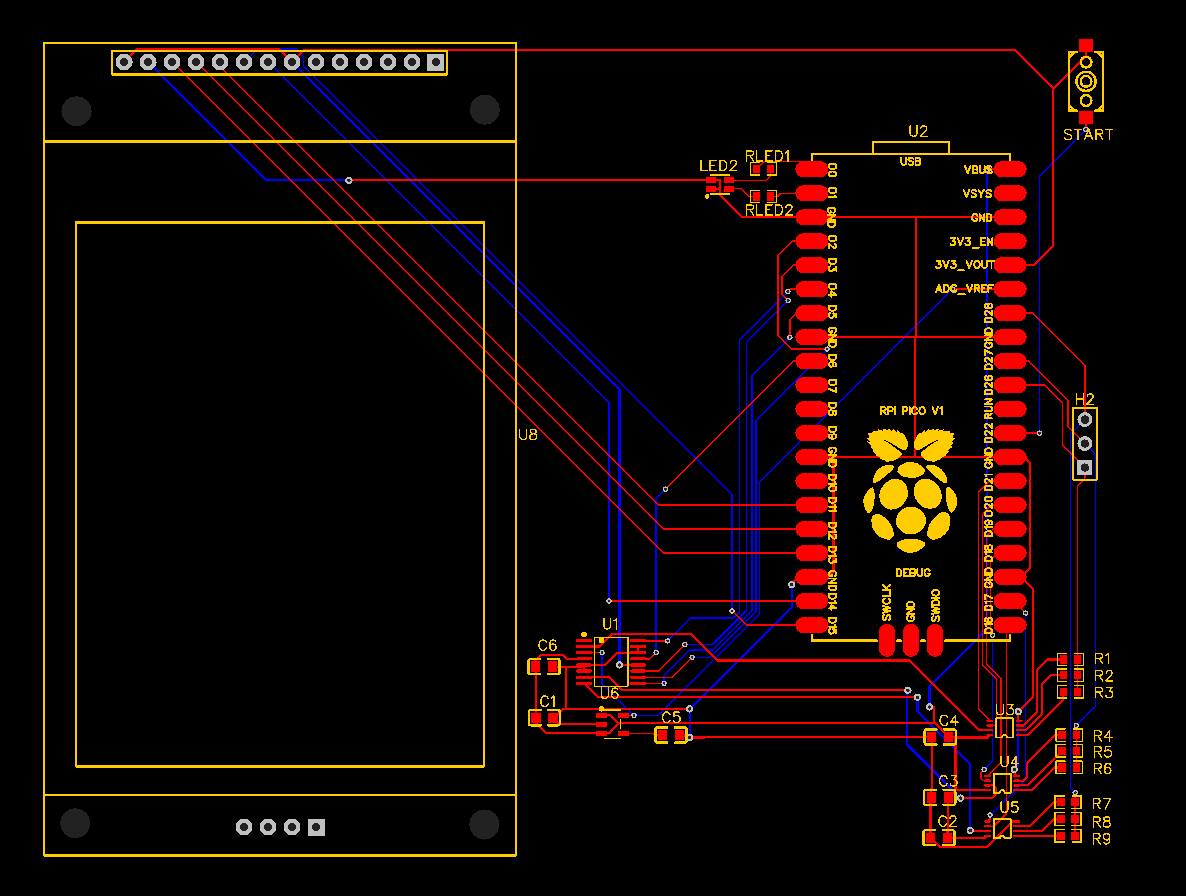
\includegraphics[scale=0.3]{images/literature/PCBV1.png}
    \caption{NYÁK első verziója}
    \label{fig:PCBV1}
\end{figure}

Legelső alkalommal a rendszer nem volt kivitelezhető, mivel túl vékony vezetékeket
használtam, ami nem volt legyártható a számomra elérhető helyeken. A komponenseket 
nehezen lehetett volna beilleszteni (Through Hole komponensek esetén, mint a kijelző),
mivel a vezetékek a lap mindkét oldalán voltak vezetve, így forrasztás során nehéz
lett volna azokat a lábakat forrasztani, amelyek a képernyő oldalán voltak.
Ezek át kellett vezessem olyan módon, hogy csakis a lap másik oldalán legyen a vezeték
csatlakoztatva a komponenshez.

Beszerzés során nem rendeltem meg minden alkatrészt, csak a fontosakat, így néhány
egyszerű alkatrészt helyettesítettem más alaktrésekkel, ez csupán egy feszültség referenciát
2 LED-et és egy kapcsolót érintett, így ezeket inkább helyileg helyettesítettem, minthogy
ismét rendeljem meg azokat.

A kijelző mérete a szerkesztőben és a valóságban nem egyezett meg, viszont ez még 
kiderült az áramkör kinyomtatása előtt, így nem vesztődött el sok idő. Az egész
kijelző nagyobb volt, mint a valóságban, még a láb közei is, így könnyedén látható
volt, hogy a tervrajz nem lesz kivitelezhető.

A tervrajzra nem tüntettem fel néhány jelzést, ami a felhasználást segíti, így ezt 
utólag felrajzoltam a lapra.

\subsection{Áramkör elkészítése}

Miután a tervezés elkészült és kivitelezhetőnek lett minősítve[\ref{fig:PCBV2}] azután az áramkör
el lett keszítve az egyetemi laboratórium segítségével. Miután a lapot a furatokkal és a réz
huzalozással megkaptam azután elkezdtem a komponensek felhelyezését.

\begin{figure}[h]
    \centering
    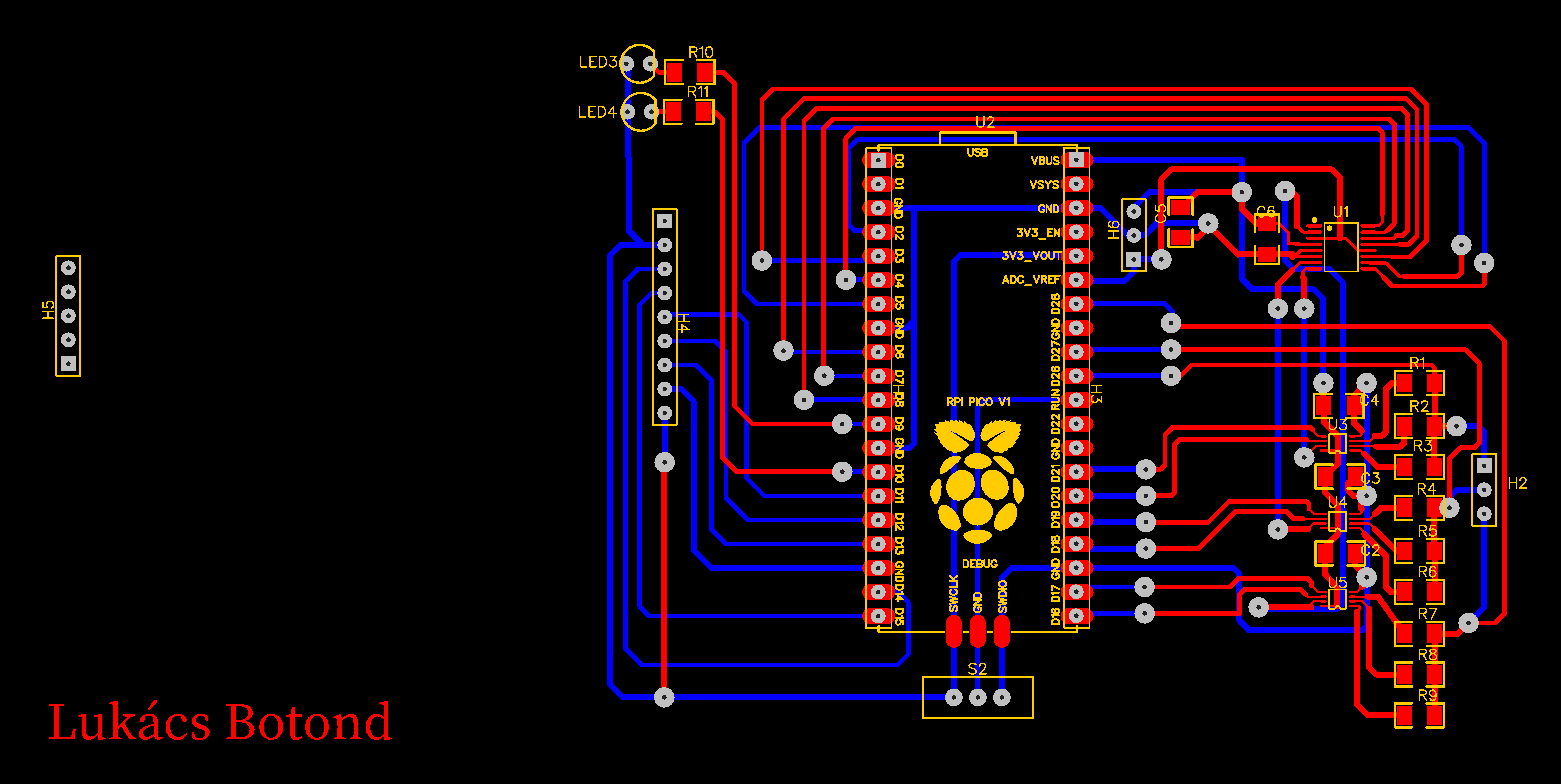
\includegraphics[scale=0.3]{images/literature/PCBV2.png}
    \caption{NYÁK végső verziója}
    \label{fig:PCBV2}
\end{figure}


Áramkör forrasztásával szintén nem volt sok tapasztalatom, csupán egyszerűbb
áramkörökkel, így nem a lehető legszebb, viszont használat során minden elektonikailag
csatlakoztatva van, így az áramkör működőképes. A végső áramkör a következőkben néz ki.
[\ref{fig:Aramkor}]


\begin{figure}[H]
    \centering
    \includegraphics[scale=0.1]{images/literature/PCB.jpg}
    \caption{A kész áramkör}
    \label{fig:Aramkor}
\end{figure}

\section{Szimulációk}

A szimulációra az LTspice \cite{LTspice} alkalmazást használtam, 
amelyben felépítettem a mérő áramkört és ellenőriztem, hogy az elméleti
mérési módszer alkalmas-e a mérés elvégzésére, és az értékek milyen
tartományban vannak, mivel a rendszer nem eléggé érzékeny, hogy a precíz
értékeket pontosan megadja, így olyan módszer kell ahol a tolerancia nagyobb.
Egy ilyen példa az áramerősség mérése amit a port ellenállást használja az
áramerősség meghatározására, viszont kis ellenállás esetén a
feszültség esés az ellenálláson alacsony áram esetén nem mérhető pontosan.
Ezért ilyen esetben nagyobb port ellenállást kell alkalmazni, hogy mérhető 
legyen a feszültség esés.

A program képes az időben változó feszültségeket is mérni, így
meg lehet tudni, hogy milyen idő intervalumban kell nézni és hogy
a komponensek időben mennyire befolyásolják a mérést. Ez 
legfőképpen a kondenzátorok mérésekor volt fontos, hogy megbizonyodjak
a mérések valóságosságáról.

A szimulációk többször is segítséget jelentettek a program 
hibáinak felfedezésében amit annélkül nehezebb lett volna felfedezni.

